\newpage
 \section{\textsc{APPIFOOD: Mobile Application for ordering and posting Foods }}
 \begin{center}
 	\textbf{}
 \end{center}
\label{chap:01}
\rhead{\itshape Mobile Application for delivering Foods }
 \lhead{}
 \cfoot{ \thepage}
  \pagestyle{fancy}
\renewcommand{\headrulewidth}{0.4pt}
%\renewcommand{\footrulewidth}{0.4pt}



\begin{flushright}
\textit{"You don’t need a silver fork to eat good food"\\
Paul Prudhomme}\\

\end{flushright}

\section{ AAAAAAAAAAAAAAAAAAAAAAAA}
\subsection{bbbbbbbbbbbbbb}
\subsubsection{ccccccccccccccccccccc}

\begin{enumerate}
    \item eeeeeeeeeeeeeeeeeeeeeeeeee
    \begin{itemize}
    \item jjjjjjjjjjjjj
    \item ppppppppppppppppppppppppppp
\end{itemize}
    \item rrrrrrrrrrrrrrrrrrrrrrrrrr
    \item ooooooooooooooooooooooooo \cite{telli}
\end{enumerate}

$$ x+y=5  $$

\PARstart With the increasing popularity of the idea of delivering food to restaurants, as well as the idea of searching for ways of comfort and luxury that people look for in their daily lives, as well as with the large number of occasions such as birthdays and weddings ... where the idea of food delivery has become the best and most effective solution in reducing the inconvenience rate among customers. As well as companies and restaurants are helping in the development and implementation of this idea. Where the idea of food delivery is an idea for companies to change their policies, orientations and marketing methods for their products.
 This idea is represented in the form of using mobile applications and it is very useful especially for restaurants to increase interaction with customers and work to improve the service, and provide information about statistics, feedback on the quality of the dishes. Our (\textbf{APPIFOOD}) online  ordering and posting food app is designed for its flexibility and high performance .
Our project aims to guide customers and consumers to follow the necessary steps in order to apply to order food  , as well as posting food and selling it .


\newpage
\subsection{Conception Part}
In this part, we will present the general architecture of our application and display it. The conception part will be including definitions of some terms besides to presenting the process of the main operations and functions of online ordering traditional food  using  diagrams.

\subsubsection{Definitions}
\begin{itemize}
	\item \textbf{Mobile Application}:\begin{small} Mobile applications are software that is designed to perform particular tasks. These food mobile applications can be provided customers with electronic services such as looking for traditional food that available, order it, and also other different functions. These can be downloaded from diverse online app stores to operate on mobile devices\cite{4}. \end{small}
	
	
	\item \textbf{Menu}:\begin{small} Menu is the statement of food and beverage items available or provided by food establishments primarily based on consumer demand and designed to achieve organizational objectives. It represents the focal point around which components of food service systems are based. The menu is designed carefully what the outlet wants to cater for, keeping in mind the type of clientele. The main advantage of a well-planned menu is that it leads to consumer satisfaction. It also helps to motivate the employees for a responsible and successful service \cite{5}. \end{small}

	\item \textbf{E-Menu}: \begin{small}electronic menu is an interactive restaurant ordering system and innovative alternative to traditional paper menus\cite{6}. \end{small}
	\item \textbf{Traditional meal}:\begin{small}Customs and traditions define the identity of the community, as it is not possible in any way to overlook or ignore the existence of these matters, as is the feature that distinguishes society from other societies.
Traditional food is an important component of the country's culture and heritage, as it is referred to as a symbol of identity as well as contributes to international recognition and reputation and also helps transmit cultural heritage to future generations\cite{9}\cite{10}. \end{small}
\end{itemize}


\newpage
\subsubsection{System Architechture}

The overall block conceptual of the proposed system is as shown in Figures 1, 2, 3, 4 and 5, this proposed diagram consists a flow of the activities in the system , followed by description before the figure for each activity.
\begin{figure}[h]
	\centering
	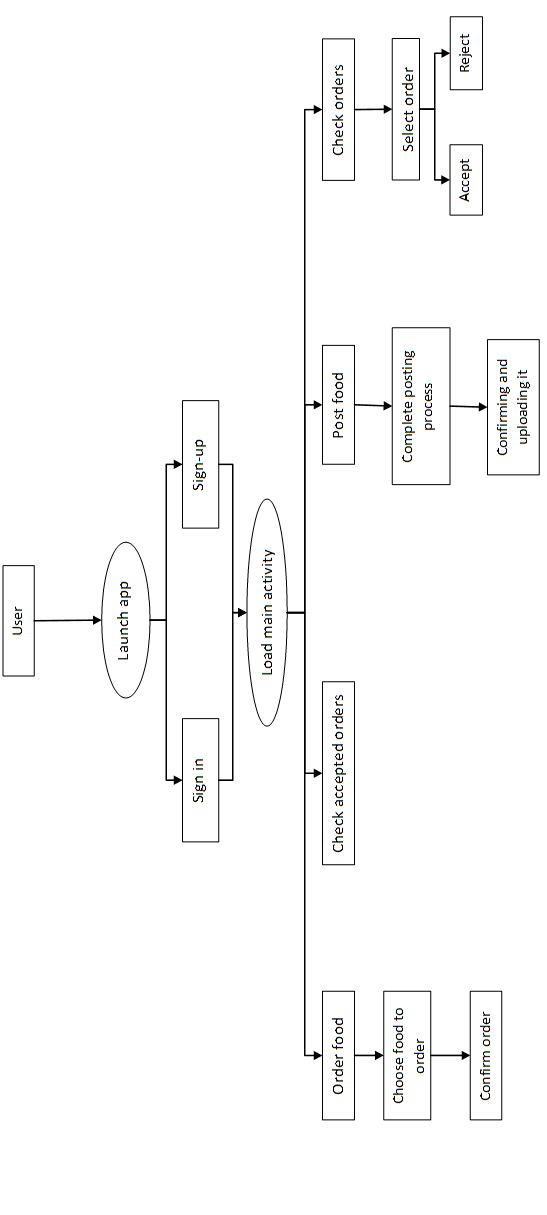
\includegraphics[width=5in,height=6.8in]{images/D1234.png}
	\caption{User Login and Registration Diagram}
\end{figure}
\newpage

\textbullet\textbf{Inscription phase:}\\
Using the app requires having an account which you can create by completing the sign-up form . In case you have an account you can use the app after logging in  by typing your login data which will be validated.

\begin{figure}[h]
	\centering
	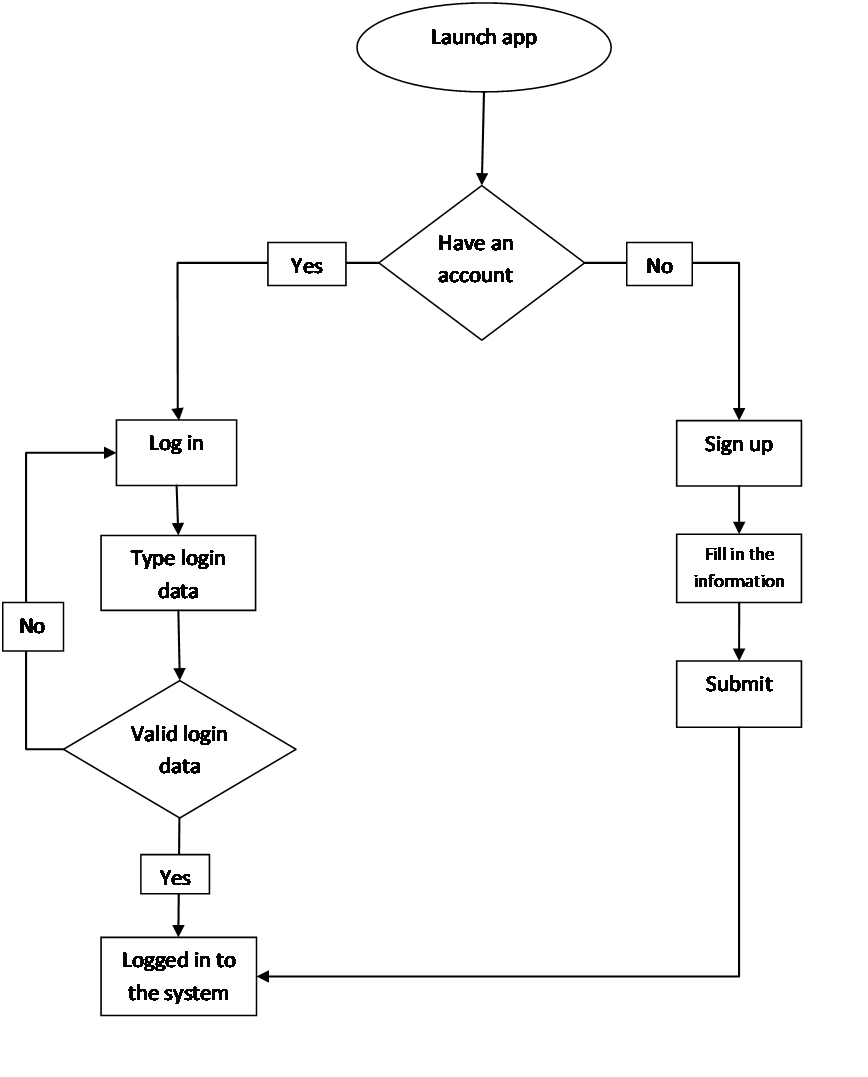
\includegraphics[width=0.8\linewidth]{images/g2.png}
	\caption{User Login and Registration Diagram}
\end{figure}
\newpage
\textbullet\textbf{Ordering phase:}\\
In this phase the user have to choose the food that he wants to order it , choose the quantity and the confirming the order which will be added to the database and sent to the owner (the user that posted the food) .
\begin{figure}[h]
	\centering
	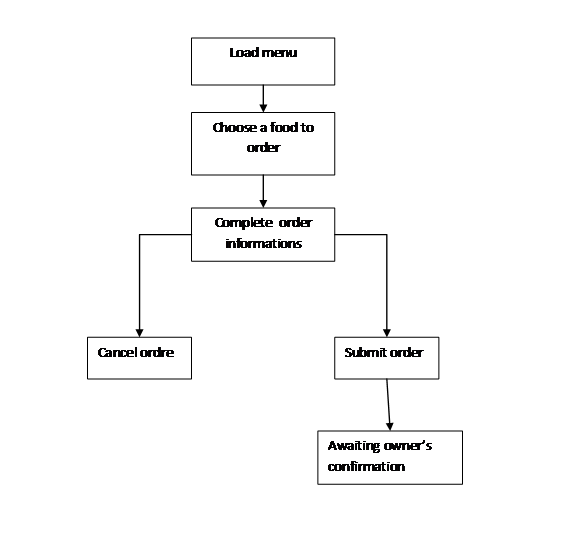
\includegraphics[width=1.0\linewidth]{images/g3.png}
	\caption{Submit Orders}
\end{figure}\\
\newpage
\textbullet\textbf{Posting Phase:}\\
In this phase users who want to sell food can add food after completing posting information (image , price , quantity ...).After that the food will be added to the database , then will be shown in the order menu . 

\begin{figure}[h]
    \centering
   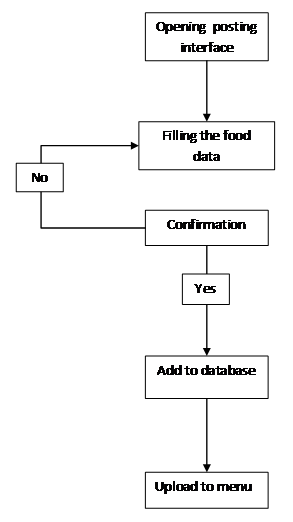
\includegraphics[width=3in,height=5in]{images/d23.png}
    \caption{posting food  Process}
    \label{fig:my_label}
\end{figure}

\textbullet\textbf{Receiving orders and accepting them:}\\
After ordering a dish , the order will be sent to the owner who can check the order then accept or delete the order .
Simultaneously , the quantity of the order will be reduced from the database .

After accepting the order the order will showed to the user that issued the order which means it has been accepted .

 \begin{figure}
 	\centering
 	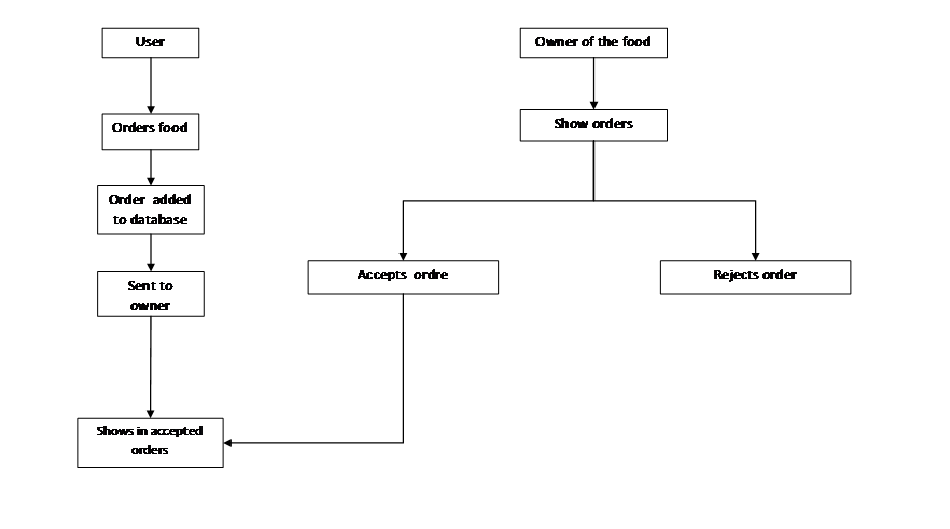
\includegraphics[width=7in,height=7in]{images/d6.png}
 	\caption{Diagram accepting orders}
 	
 \end{figure}







\newpage
\subsubsection{System Operations}
This section consists a description of the deferent tasks of each actor (admin and user)\\
 \textopenbullet \textbf{The User tasks:}\\
 There are several tasks that our application offers to the users starting with :
 


 \textleaf  \textbf{ Inscription  (sign-up):}\\
To use the app the user have to create an account by giving a necessary information (name , email , phone number ...) , after system verification the data will be registered and saved instancely in the database (Firebase realtime database) .

 \textleaf  \textbf{ Login/logout:}\\
After the inscription process the user doesn’t have to sign-up again but he will have to fill three information fields (name , password and phone number) to login to the app and access the other tasks.
After finishing using the app the user can logout from his account in case someone got his phone and tried to open the application.

 \textleaf \textbf { Home page :}\\
After login in to the account the user will be faced with three options:

\textbullet\textbf{Ordering food:}\\
From this option the user can access the menu of the added food by other users and choose the food that he want to order and the quantity . Also after choosing a dish the user can see some information about the dish and the available quantity and information about the poster (owner).

\textbullet\textbf{Posting food:}\\
From this option the user can add food to the menu of the app to sell it .
After completing a form about the food that will be added and adding a picture of the food and confirming the information the food will be added to the database and available to other users from the ordering option.

\textbullet\textbf{Managing orders :}\\
The user who sell food in this app can check if they received an order then decide whether they accept it or not , in case the accepted it the user who made the order can also check the acceptance of it from the app .   



\newpage
\subsection{Implementation Part}
In this part, the focus is on implementation of our system which makes it possible to evaluate our application. This part is including a description hardware and software needs. In addition, the mobile applications interfaces and presents the different interfaces of mobile applications realized.

\subsubsection{Hardware Description}
The programming of the application was carried out on  the followings devices:
\begin{itemize}
	\item TOSHIBA laptop\\
\textbf{Mark:} TOSHIBA \\
\textbf{RAM:} 4.00 Go\\
\textbf{Hard Disk:} 300 Go\\
\textbf{Processor:} Intel(R) Core(TM)2 Duo CPU T6400 @ 2.00GHz 2.00 GHz\\
\textbf{Exploitation System:} Windows 10 professional
\item DELL Laptop\\
\textbf{Mark:} DELL \\
\textbf{RAM:} 4.00 Go\\
\textbf{Hard Disk:} 500 Go\\
\textbf{Processor:} Processor	Intel(R) Celeron(R) N4000 CPU @1.10 GHz 1.10 GHz\\
\textbf{Exploitation System:}Ubunto
\item Mobile Phone \\
\textbf{Mark:} OPPO A1K \\
\textbf{RAM:} 2.00 Go\\
\textbf{Storage:} 32 Go\\
\textbf{Version Android:} 9
\item Mobile Phone \\
\textbf{Mark:} Galaxy J7 Duo \\
\textbf{RAM:} 4.00 Go\\
\textbf{Storage:} 32 Go\\
\textbf{Version Android:} 10
\end{itemize}

\subsubsection{Software Description}
The tools selected for the realization of the mobile application are the following: 

\begin{itemize}

\item \textbf{Android Studio 4.2.1 :}\\
\begin{small}
Android Studio is the official integrated development environment (IDE) for Google's Android operating system, built on JetBrains' IntelliJ IDEA software and designed specifically for Android development  It is available for download on Windows, macOS and Linux based operating systems or as a subscription-based service in 2020. It is a replacement for the Eclipse Android Development Tools (E-ADT) as the primary IDE for native Android application development\cite{11} .
\end{small}
\item \textbf{Java Language :}\\
\begin{small} Java is a powerful general-purpose programming language and a computing platform created by Sun Mi ecosystems in 1995. It is the underlying technology that enables the execution of modern and powerful programs, including the construction of utilities, games and professional applications. According to Oracle, the company that owns Java, Java runs on 3 billion devices worldwide, including mobile devices and television broadcasting systems, which makes Java one of the most popular programming languages\cite{12}.
\end{small}
\item \textbf{The Firebase Realtime Database  :}\\
\begin{small}
Firebase is a platform developed by Google for creating mobile and web applications. It was originally an independent company founded in 2011. In 2014, Google acquired the platform and it is now their flagship offering for app development.
The Firebase Realtime Database is a cloud-hosted database. Data is stored as JSON and synchronized in realtime to every connected client. When you build cross-platform apps with our iOS, Android, and JavaScript SDKs, all of your clients share one Realtime Database instance and automatically receive updates with the newest data
\cite{13} \cite{14}.
\newpage
\end{small}
\end{itemize}
\begin{figure}[h]
    \centering
    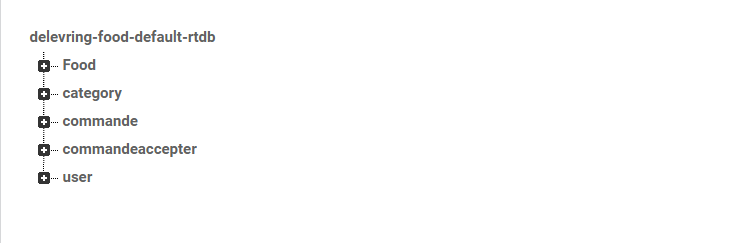
\includegraphics[width=1.5\linewidth]{images/aaa.PNG}
    \caption{database}
    \label{fig:my_label}
\end{figure}

\newpage

\subsubsection{Mobile Application Interfaces}
\begin{enumerate}
  \item \textbf{First interface:}
 
  After you launch the app you will be faced with the interface bellow.
  This interface contain two buttons one will lead to sign-up interface will the second lead to sign in interface
\begin{figure}[h]


 	\centering
 	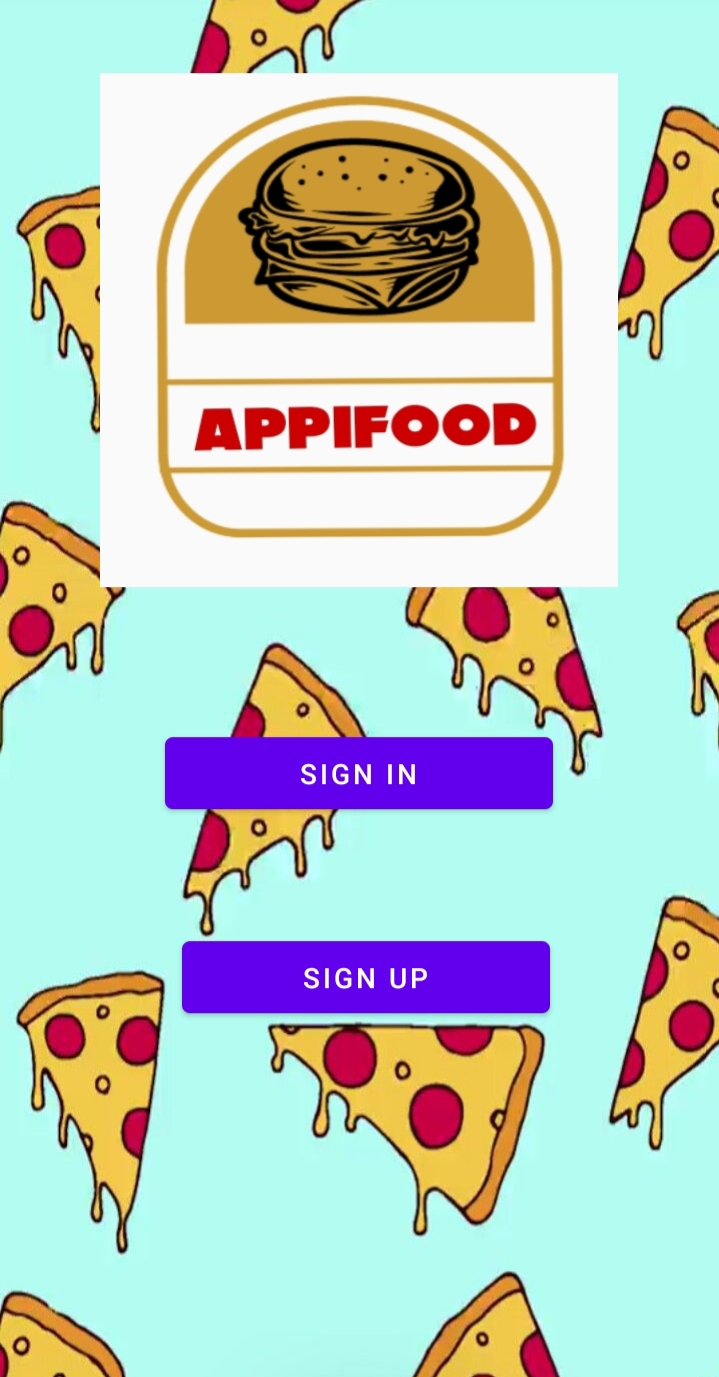
\includegraphics[width=3in,height=5in]{images/act1.jpg}
 	\caption{First interface}
 	

\end{figure}

\item \textbf{Sign in and Sign-up  Interface:}

If the user click on the sign in button , he will be directed to the interface bellow which is the Sign in "Login" interface where he can sign in directly if he has already an account. 

\begin{figure}[h]
    \centering    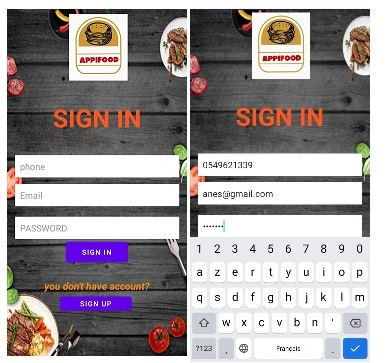
\includegraphics[width=4in,height=3in]{images/act4.jpg}
    \caption{Sign in}
    \label{fig:my_label}
\end{figure}

\newpage
Other than that ,  the user can create new account by filling the registration form with his data in the sign-up interface .
\begin{figure}[h]
    \centering    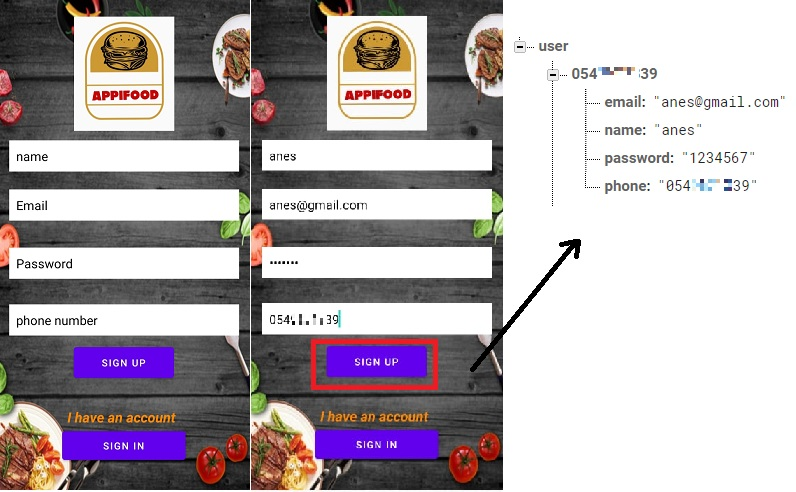
\includegraphics[width=6in,height=3in]{images/ACT6.jpg}
    \caption{Sign up}
    \label{fig:my_label}
\end{figure}

\item \textbf{Main Interface:}

In This interface which you can access after signing in or signing up , you will see four buttons ,each button lead to a different activity.
\newpage
\begin{figure}[h]
    \centering
   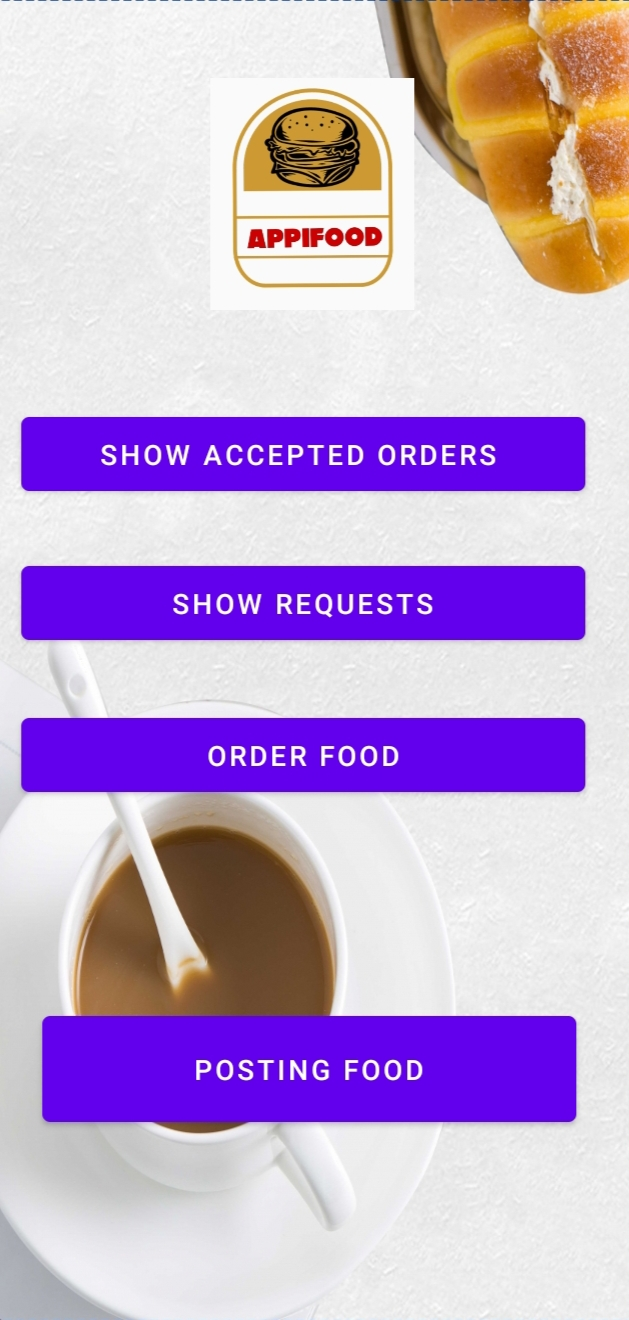
\includegraphics[width=2in,height=3in]{images/act4btn.jpg}
    \caption{Main Interface}
    \label{fig:my_label}
\end{figure}

 \item \textbf{Menu and order interface:}
 
 After clicking "order food"  button ,the app will send the user to menu interface where he can see the food posted by users.
 
 \begin{figure}[h]
    \centering
   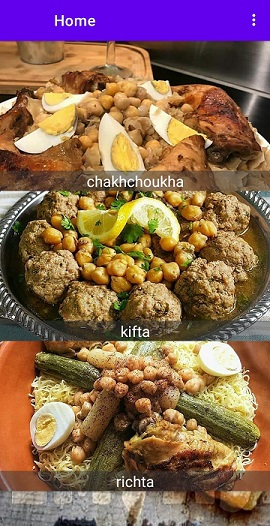
\includegraphics[width=2in,height=3.1in]{images/actorder2.jpg}
    \caption{Menu Interface}
    \label{fig:my_label}
\end{figure}
If the user clicked on a picture of a food he can see the price , the phone of the owner and available quantity.Also he will see 2 fields for his phone number and the quantity he want to buy . 
After filling the two fields and clicking the order button a confirmation me will appear , asking the user whether he is sure of his order or not .
Then the command will be added to the database , then sent to the owner .
\begin{figure}[h]
    \centering
   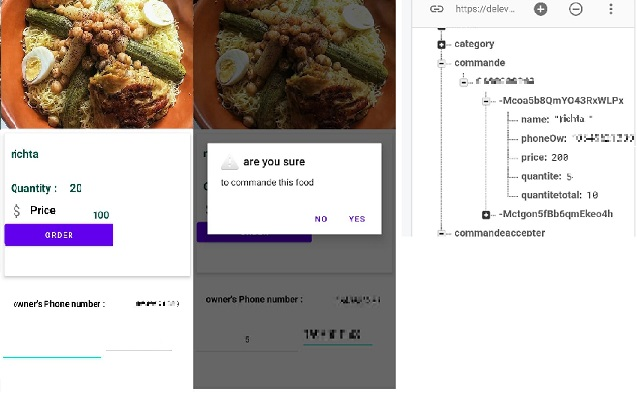
\includegraphics[width=6.5in,height=3in]{images/act12.jpg}
    \caption{order Process}
    \label{fig:my_label}
\end{figure}

\item \textbf{Posting food interface:}

In this interface we represent to the users the ability to post their own food to sell .
\begin{figure}[h]
    \centering
   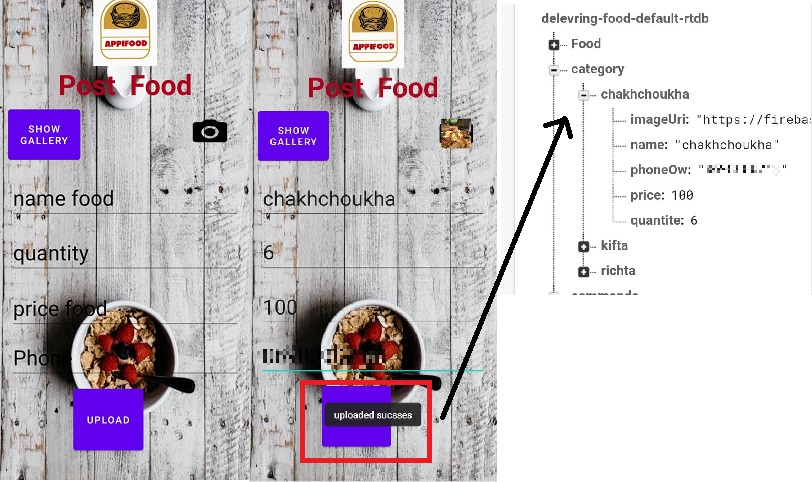
\includegraphics[width=6in,height=3in]{images/actpost2.jpg}
    \caption{Posting Process}
    \label{fig:my_label}
\end{figure}
\newpage
\item \textbf{Accepting orders interface:}

After an order have been issued by a user , the owner receive  the and he can check it by entering the "show requests"  , there he will faced with the requests of users of the food he posted . Then , he can accept by clicking on the request which will show a message that have two options "Accept" or "Delete" .
\begin{figure}[h]
    
   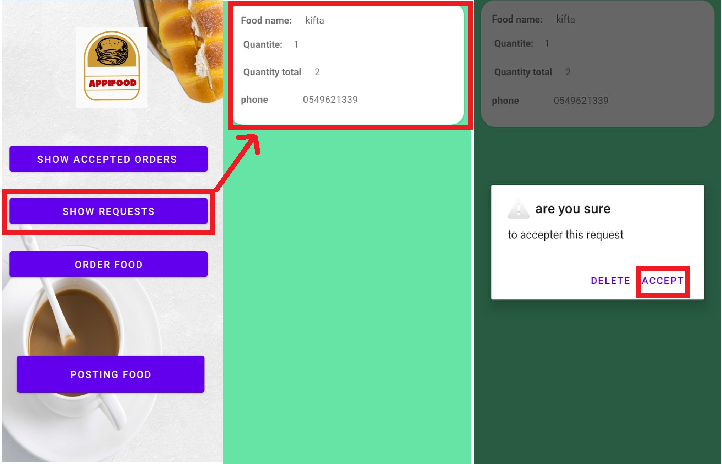
\includegraphics[width=1\linewidth,height=4in]{images/ACT13.png}
    \caption{Accepting  Process}
    \label{fig:my_label}
\end{figure}

\item \textbf{After Accepting orders:}

This part describes what happens after accepting an order.
The user who issued the order will be able to see his order after clicking on show accepted orders which means his order has been approved by the owner.

Simultaneously , after the order has been accepted the quantity of the dish will be reduced . 
 \newpage    

\begin{figure}[h]
    \centering
   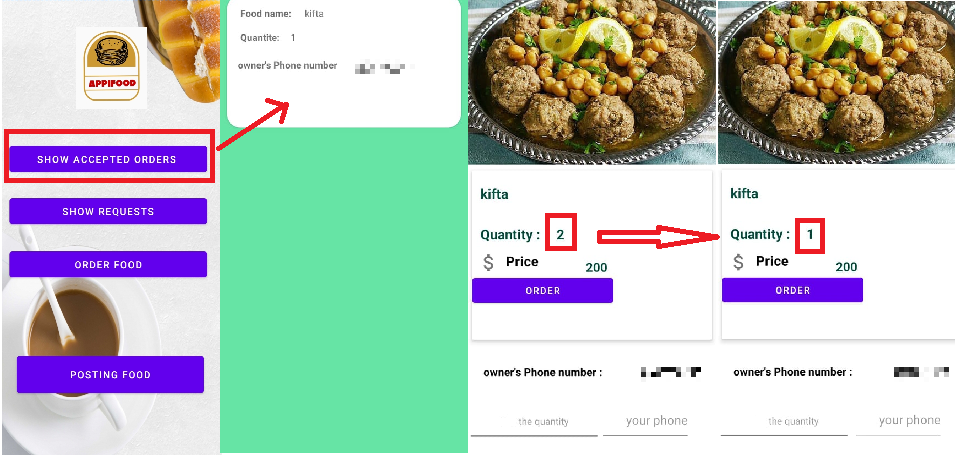
\includegraphics[width=6.5in,height=3.5in]{images/ACT14.png}
    \caption{After Accepting order Process}
    \label{fig:my_label}
\end{figure}

\end{enumerate}
 \newpage    

    
    



























